\documentclass[aspectratio=169]{beamer}
\usepackage{tikz}
\usetikzlibrary{positioning,arrows.meta}
\usepackage{amsmath}
\usepackage{xcolor}
\setbeamertemplate{navigation symbols}{}
\definecolor{navy}{RGB}{20,37,63}
\definecolor{blue2}{RGB}{44,118,190}
\definecolor{gold}{RGB}{235,170,48}
\definecolor{light}{RGB}{245,248,252}
\setbeamercolor{normal text}{fg=navy,bg=white}
\setbeamercolor{frametitle}{fg=navy}
\setbeamerfont{frametitle}{series=\bfseries,size=\Large}

\newcommand{\card}[4]{%
  \fill[#1,rounded corners=5pt] (#2) rectangle (#3);%
  \node[anchor=north west,text width=#4] at (#2) {\strut};%
}

\begin{document}
\begin{frame}[t]
\frametitle{Segment Tree}
\framesubtitle{Fast range queries + point updates in $O(\log n)$}

\begin{columns}[T,totalwidth=\textwidth]
\column{0.49\textwidth}
\begin{block}{Core idea}
A segment tree stores information for \textbf{intervals} of an array.
\begin{itemize}\itemsep3pt
  \item Each node represents a segment $[l,r]$.
  \item Internal node = merge(left child, right child).
  \item Leaves represent single elements.
\end{itemize}
\end{block}

\vspace{5pt}
\begin{exampleblock}{Example: range sum}
For $A=[2,1,5,3]$:\\[-2pt]
root stores $2+1+5+3=11$.
\end{exampleblock}

\vspace{4pt}
\begin{alertblock}{Complexity}
Build: $O(n)$ \quad Query: $O(\log n)$ \quad Update: $O(\log n)$
\end{alertblock}

\column{0.51\textwidth}
\centering
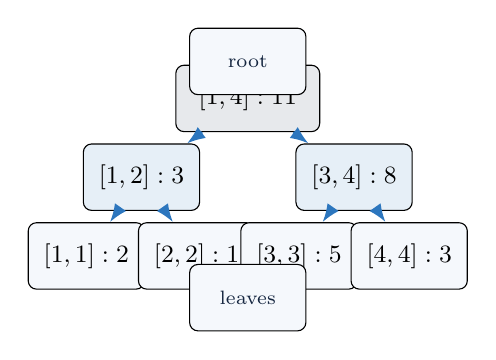
\begin{tikzpicture}[
  every node/.style={draw,rounded corners=3pt,minimum width=42pt,minimum height=24pt,font=\small,fill=light},
  edge/.style={-Latex,thick,draw=blue2},
  lvl/.style={font=\scriptsize\color{navy}}
]
\node[fill=navy!10,minimum width=52pt] (r) at (0,2.25) {$[1,4]:11$};
\node[fill=blue2!12] (a) at (-1.35,1.25) {$[1,2]:3$};
\node[fill=blue2!12] (b) at (1.35,1.25) {$[3,4]:8$};
\node (c) at (-2.05,0.25) {$[1,1]:2$};
\node (d) at (-0.65,0.25) {$[2,2]:1$};
\node (e) at (0.65,0.25) {$[3,3]:5$};
\node (f) at (2.05,0.25) {$[4,4]:3$};
\draw[edge] (r)--(a); \draw[edge] (r)--(b);
\draw[edge] (a)--(c); \draw[edge] (a)--(d);
\draw[edge] (b)--(e); \draw[edge] (b)--(f);
\node[lvl] at (0,2.72) {root};
\node[lvl] at (0,-0.28) {leaves};
\end{tikzpicture}

\vspace{2pt}
\begin{block}{How a query works}
Decompose $[L,R]$ into a small number of tree segments, then merge their values.
\end{block}

\end{columns}

\vfill
\begin{center}
\footnotesize\textcolor{navy!70}{\textbf{CSE200 — LaTeX Course} \hspace{8pt}|\hspace{8pt} Data Structures}\qquad
\textcolor{gold}{\rule{34pt}{1.4pt}}
\end{center}
\end{frame}
\end{document}
